% ICLR two-column motivation figure; requires graphicx.
\begin{figure*}[t]
  \centering
  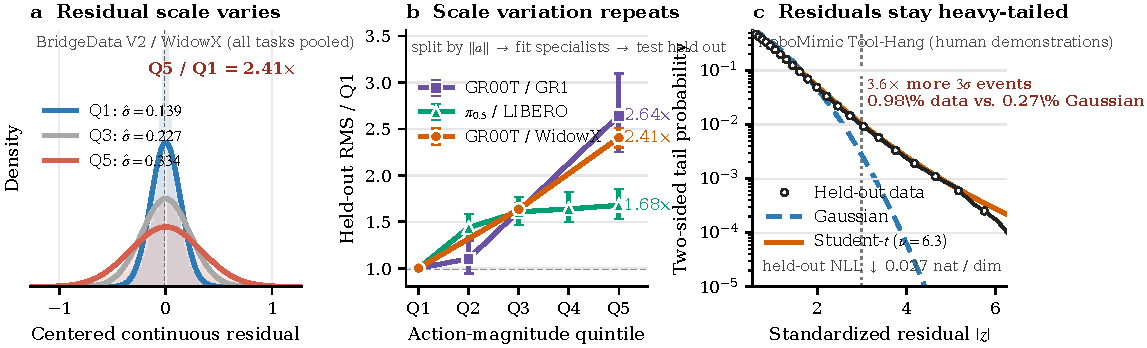
\includegraphics[width=\textwidth]{analysis/paper/action_magnitude_specialists/fig_split_fit_scale.pdf}
  \caption{\textbf{Robot action residuals exhibit input-dependent scales and
  heavy tails.}
  We partition the training demonstrations into quintiles of normalized
  continuous-action magnitude, fit an independent MSE specialist to each
  quintile, and evaluate each specialist only on matching held-out episodes.
  \textbf{(a)} Empirical coordinate-residual histograms over all held-out
  BridgeData V2/WidowX tasks, after coordinate-wise centering, and zero-mean
  Gaussian fits with the measured radii. The Q5 residual radius is
  $2.41\times$ the Q1 radius.
  \textbf{(b)} Held-out residual RMS relative to Q1 increases by
  $2.64\times$ on GR1, $1.68\times$ on LIBERO, and $2.41\times$ on WidowX.
  Error bars are 95\% cluster-bootstrap intervals over tasks for GR1 and
  LIBERO and over episodes for WidowX.
  \textbf{(c)} On held-out human Tool-Hang demonstrations, residuals remain
  heavy-tailed after normalization by state-local and per-coordinate RMS:
  $P(|z|>3)$ is $0.98\%$, versus $0.27\%$ under a Gaussian. A cross-fitted
  Student-$t$ ($\nu=6.3$) follows the empirical tail and reduces held-out NLL
  by $0.027$ nat per action dimension. Binary gripper channels are excluded
  for LIBERO, WidowX, and Tool-Hang; GR1 retains its continuous hand joints.}
  \label{fig:split-fit-scale}
\end{figure*}
